\chapter{Comparison of Regularized Density Estimators in Kernel Exponential Families}
\label{ch4}

After discussing the early stopping SM density estimator and comparing it with the penalized SM density estimator in the preceding chapter, we now turn to comparing these two kinds of regularized SM density estimators with the penalized ML density estimator. In particular, we would like to understand what differences the regularized SM density estimators and the penalized ML density estimator have and why they have such differences. 

In Section \ref{section-ml-density-estimator}, we focus on the penalized ML density estimator. We will establish the existence and the uniqueness of the minimizer of the penalized NLL loss functional. In spite of its existence, similar to the discussion in Chapter \ref{ch2} and that by \textcite{Gu1993-na}, such a minimizer in an infinite-dimensional RKHS is computationally intractable. Instead, we seek a finite-dimensional subspace of $\calH$ to approximate this minimizer. In order to ensure the comparability of SM and ML density estimators, we minimize the (penalized) SM loss functional over this finite-dimensional subspace as well, and discuss how to compute the penalized and early stopping SM density estimators in it in Section \ref{section-computation-sm-density-estimator}. We then discuss the similarities and differences between regularized SM density estimators and penalized ML density estimator via numerical examples in Section \ref{section-ml-sm-comparison}. Finally, we explain why they have the observed differences in Section \ref{section-sm-explanation}. 

\section{Penalized Maximum Likelihood Density Estimator}\label{section-ml-density-estimator}

In this section, we look at the penalized ML density estimator, which is obtained by minimizing 
\begin{align}\label{eq-pen-nll-loss}
	\widehat{J}_{\NLL} \parens{f} + \frac{\lambda}{2} \norm{f}_{\calH}^2, \qquad \text{ subject to } f \in \calF, 
\end{align}
where $\widehat{J}_{\NLL} \parens{f} = A \parens{f} - \frac{1}{n} \sum_{i=1}^n f \parens{X_i}$ is the NLL loss functional we have seen in Chapter \ref{ch2}, and $\lambda \ge 0$ is the penalty parameter. Note that in \eqref{eq-pen-nll-loss}, we choose the penalty functional to be $\widetilde{P} \parens{f} := \frac{1}{2} \norm{f}_{\calH}^2$, for all $f \in \calH$, which is to ensure the comparability with the regularized SM density estimators. 

The following proposition established the existence and the uniqueness of the minimizer of \eqref{eq-pen-nll-loss}. 

\begin{proposition}\label{prop-nll-sol-exist-unique}
	Under Assumptions \ref{assumption-2-1-inf-dim} - \ref{assumption-2-4-base-density} in Chapter \ref{ch2}, for every $\lambda > 0$, \eqref{eq-pen-nll-loss} has a unique minimizer in $\calF$. 
\end{proposition}

The proof of Proposition \ref{prop-nll-sol-exist-unique} is given in Section \ref{proof-prop-nll-sol-exist-unique}. 

\subsection{Failure of the Representer Theorem}

Note that Proposition \ref{prop-nll-sol-exist-unique} only shows \eqref{eq-pen-nll-loss} has a unique minimizer, but gives no indication what such a minimizer is like. 

Since minimizing \eqref{eq-pen-nll-loss} is a convex minimization problem over an infinite-dimensional RKHS, a classic tool of characterizing its minimizer is the representer theorem \parencite{Kimeldorf1971-lf,Scholkopf2001-bb}, which states that, if $\widetilde{J}: \calH \to \Real$ is a convex loss functional that depends \emph{only} on the evaluation of $f \in \calH$ at data points $X_1, \cdots, X_n$, then 
\begin{align*}
	\min_{f \in \calH} \braces[\bigg]{\widetilde{J} \parens{f} + \frac{\lambda}{2} \norm{f}_{\calH}^2} = \min_{f \in \mathrm{Span} \sets{k \parens{X_1, \,\cdot\,}, \cdots, k \parens{X_n, \,\cdot\,}}} \braces[\bigg]{\widetilde{J} \parens{f} + \frac{\lambda}{2} \norm{f}_{\calH}^2}; 
\end{align*}
in other words, the minimizer of $\widetilde{J} \parens{f} + \frac{\lambda}{2} \norm{f}_{\calH}^2$ over $\calH$ can be represented as a linear combination of $k \parens{X_1, \,\cdot\,}, \cdots, k \parens{X_n, \,\cdot\,}$. Here, we only consider a specific form of the penalty functional $\frac{\lambda}{2} \norm{f}_{\calH}^2$. The representer theorem covers the case where a general penalty functional is used; see \textcite{Scholkopf2001-bb} for a discussion. 

The representer theorem is a powerful tool and reduces a convex minimization problem in an infinite-dimensional RKHS to the one in a finite-dimensional subspace, which effectively reduces the computational burden and improves the efficiency. However, note that, due the presence of $A$ in \eqref{eq-pen-nll-loss}, $\widehat{J}_{\NLL}$ does not only depend on the evaluation of $f$ at data points $X_1, \cdots, X_n$, but also on that of $f$ at \emph{all} points in $\calX$. This suggests the representer theorem may fail in characterizing the minimizer of \eqref{eq-pen-nll-loss}. In fact, as the following example demonstrates, the representer theorem does fail. 

\begin{example}\label{example-representer-theorem-fails}
	Let $\calX = \Real^2$ and the kernel function be $k \parens{x, y} = \parens{x^\top y}^2$ for all $x, y \in \Real^2$, i.e., the homogeneous polynomial kernel of degree 2. We choose the base density to be $\mu \parens{x} = \frac{1}{2 \pi} \exp \parens{-\frac{\norm{x}_2^2}{2}}$ for all $x \in \Real^2$, i.e., the pdf of 2-dimensional Gaussian distribution with the zero mean and the identity covariance matrix. We fix $n = 1$ and let the single data point be $X_1 = \parens{a, 0}^\top \in \Real^2$. Also, let $\lambda > 0$. 
	
	Then, it can be shown that the minimizer of the corresponding penalized NLL loss functional 
	\begin{align}\label{eq-example-nll-representer-theorem-fails-1}
		A \parens{f} - f \parens{X_1} + \frac{\lambda}{2} \norm{f}_{\calH}^2, \qquad \text{ subject to } f \in \calF, 
	\end{align}
	takes on the form of 
	\begin{align*}
		f^* \parens{x} = b^* x_1^2 + c^* x_2^2, \qquad \text{ for all } x = \parens{x_1, x_2}^\top \in \Real^2, 
	\end{align*}
	for some $b^* \neq 0$ and $c^* \neq 0$, but $\mathrm{Span} \braces{k \parens{X_1, \,\cdot\,}} \cap \calF$ contains all functions of the form
	\begin{align*}
		f \parens{x} = \gamma a^2 x_1^2, \quad \text{ for all } x := \parens{x_1, x_2}^\top \in \Real^2 \text{ and } \gamma \in \Real \text{ satisfying } \gamma a^2 < \frac{1}{2}. 
	\end{align*}
	Thus, $f^* \notin \mathrm{Span} \braces{k \parens{X_1, \,\cdot\,}} \cap \calF$ and we conclude the representer theorem fails. 
		
	Details about this example can be found in Section \ref{proof-example-representer-theorem-fails}. 
\end{example}


\subsection{Construction of a Finite-dimensional Approximating Space}

Now, we have seen the representer theorem fails in characterizing the minimizer of \eqref{eq-pen-nll-loss}. In addition, as we have discussed in Chapter \ref{ch2}, despite its existence and uniqueness, such a minimizer in an infinite-dimensional $\calH$ is computationally intractable. In order to compute the penalized ML density estimator, we propose to seek a finite-dimensional subspace in $\calH$ to approximate the minimizer of \eqref{eq-pen-nll-loss}, which is the focus of the current section. 

One idea is to choose the following $n$-dimensional subspace spanned by the kernel functions centered at $X_1, \cdots, X_n$, 
\begin{align}\label{eq-fin-approx-subspace-gu-qiu}
	\sets[\Bigg]{f \biggm| f := \sum_{i=1}^n \beta_i k \parens{X_i, \,\cdot\,}, \beta_1, \cdots, \beta_n \in \Real}, 
\end{align}
as the approximating space. This is the approach taken by \textcite{Gu1993-na} and \textcite{Gu1993-lf}. 

We propose a different approach here. Suppose $\calX \subseteq \Real$ for the moment and start with a set of grid points over $\calX$, denoted by $\bX_1 := \sets{w_1, \cdots, w_m}$, that covers the range of data. We minimize the objective functional in \eqref{eq-pen-nll-loss} over 
\begin{align*}
	\widetilde{\calH}_1 := \sets[\Bigg]{f \biggm| f := \sum_{j=1}^{m} \beta_j k \parens{w_j, \,\cdot\,}, \beta_j \in \Real, w_j \in \bX_1, \text{ for all } j = 1, \cdots, m}. 
\end{align*}
Then, we insert an additional grid point at the midpoint of two adjacent points in $\bX_1$, forming 
\begin{align*}
	\bX_2 := \sets[\Big]{w_1, w_{1.5}, w_{2}, \cdots, w_{m-1}, w_{\frac{2m-1}{2}}, w_m}, 
\end{align*}
where $w_{\frac{2j-1}{2}} = \frac{1}{2} \parens{w_{j} + w_{j+1}}$ for all $j = 1, \cdots, m-1$, and minimize \eqref{eq-pen-nll-loss} over 
\begin{align*}
	\widetilde{\calH}_2 := \sets[\Bigg]{f \biggm| f := \sum_{j \in \sets{1, 1.5, 2, \cdots, m}} \beta_j k \parens{w_j, \,\cdot\,}, \beta_j \in \Real, w_j \in \bX_2, \text{ for all } j = 1, 1.5, 2, \cdots, m}. 
\end{align*}
Let $\tilde{f}_{\ML, \ell} := \argmin_{f \in \widetilde{\calH}_{\ell}} \sets[\big]{\widehat{J}_{\NLL} \parens{f} + \frac{\lambda}{2} \norm{f}_{\calH}^2}$ for $\ell = 1, 2$. Then, we compute the following relative difference 
\begin{align}\label{eq-termination-grid-points}
	\abs[\Bigg]{\frac{ \bracks[\big]{\widehat{J}_{\NLL} \parens{\tilde{f}_{\ML, 2}} + \frac{\lambda}{2} \norm{\tilde{f}_{\ML, 2}}_{\calH}^2} - \bracks[\big]{\widehat{J}_{\NLL} \parens{\tilde{f}_{\ML, 1}} + \frac{\lambda}{2} \norm{\tilde{f}_{\ML, 1}}_{\calH}^2 } }{\widehat{J}_{\NLL} \parens{\tilde{f}_{\ML, 1}} + \frac{\lambda}{2} \norm{\tilde{f}_{\ML, 1}}_{\calH}^2 } }. 
\end{align}
Since $\bX_1 \subset \bX_2$ and $\widetilde{\calH}_1 \subset \widetilde{\calH}_2$, we must have $\widehat{J}_{\NLL} \parens{\tilde{f}_{\ML, 1}} + \frac{\lambda}{2} \norm{\tilde{f}_{\ML, 1}}_{\calH}^2 \ge \widehat{J}_{\NLL} \parens{\tilde{f}_{\ML, 2}} + \frac{\lambda}{2} \norm{\tilde{f}_{\ML, 2}}_{\calH}^2$. 

We repeat the process described above: keep inserting additional grid points at the midpoint of two adjacent points, minimize the penalized NLL loss functional over the new finite-dimensional subspace with the updated grid points, and stop until the relative difference of the values of the penalized NLL loss functional between two consecutive sets of grid points does not exceed a pre-specified tolerance parameter. The algorithm is provided in Algorithm \ref{algo-determine-approximate-space}. 

\begin{algorithm}
\caption{Determining the finite-dimensional subspace of approximating the minimizer of $\widehat{J}_{\NLL} \parens{f} + \frac{\lambda}{2} \norm{f}_{\calH}^2$ over $f \in \calH$}\label{algo-determine-approximate-space}
\begin{algorithmic}[1]
\Statex \algorithmicrequire 
\begin{itemize}\setlength\itemsep{0em}
	\item $X_1, \cdots, X_n$, the data from $p_0$; 
	\item $\bX_1 := \sets{w_1, \cdots, w_m}$, the first set of grid points; 
	\item $\epsilon > 0$, the tolerance parameter. 
\end{itemize}

\vspace{5pt}

\State Let $\widetilde{\calH}_{1} = \sets[\big]{f \mid f := \sum_{j} \beta_j k \parens{w_j, \,\cdot\,}, \beta_j \in \Real, w_j \in \bX_1, \text{ for all } j = 1, 2, \cdots, m}$ and compute $\tilde{f}_{\ML, 1} := \argmin_{f \in \widetilde{\calH}_1} \sets[\big]{\widehat{J}_{\NLL} \parens{f} + \frac{\lambda}{2} \norm{f}_{\calH}^2}$; 
\State Form $\bX_2$, which is obtained by adding a grid point at the midpoint of two adjacent points in $\bX_1$; 
\State Compute $\tilde{f}_{\ML, 2} := \argmin_{f \in \widetilde{\calH}_2} \sets[\big]{\widehat{J}_{\NLL} \parens{f} + \frac{\lambda}{2} \norm{f}_{\calH}^2}$, where $\widetilde{\calH}_2 := \sets{f \mid f := \sum_{j} \beta_j k \parens{w_j, \,\cdot\,}, \beta_j \in \Real, w_j \in \bX_2}$; 
\State Compute $\mathtt{error}$ using \eqref{eq-termination-grid-points}; 
\While{$\mathtt{error} > \epsilon$}
\State Let $\bX_1 = \bX_2$, and form a new $\bX_2$ by adding a grid point at the midpoint of two adjacent points in $\bX_1$; 
\State Let $\tilde{f}_{\ML, 1} = \tilde{f}_{\ML, 2}$, and compute $\tilde{f}_{\ML, 2} := \argmin_{f \in \widetilde{\calH}_2} \sets[\big]{\widehat{J}_{\NLL} \parens{f} + \frac{\lambda}{2} \norm{f}_{\calH}^2}$, where $\widetilde{\calH}_2 := \sets{f \mid f := \sum_{j} \beta_j k \parens{w_j, \,\cdot\,}, \beta_j \in \Real, w_j \in \bX_2}$; 
\State Update $\mathtt{error}$ using \eqref{eq-termination-grid-points}. 
\EndWhile
\State \Return $\bX_{1}$. 
\end{algorithmic}
\end{algorithm}


If $\calX \subseteq \Real^d$ for $d > 1$, we can generalize the procedure described above accordingly. However, one has to be careful when adding additional points, since, with $d > 1$, each grid point has up to $2^d$ adjacent points, and the number of grid points being added each time can grow exponentially. The computational burden will also increase accordingly as $d$ increases. This is one example of the infamous curse of dimensionality and is an unsatisfactory feature of our approach. 

One advantage of our approach, comparing to the approach by \textcite{Gu1993-na} and \textcite{Gu1993-lf}, is that our approach can yield an even smaller minimum of the penalized NLL loss functional than theirs, as we will see via numerical examples in Section \ref{subsubsubsection-illustration-fin-dim-appro-space}. 

In our description of the process above, one key component we have not discussed is how to compute the minimizer of the penalized NLL loss functional for a given finite-dimensional approximating subspace. As we have discussed in Chapter \ref{ch2}, the main difficulty is to handle $A$ and its derivatives efficiently. In the next section, we propose an algorithm to approximate the values of $A$ and its derivatives and compute the minimizer of the penalized NLL loss functional. 

\begin{remark}
	An alternative subspace we can use to approximate the minimizer of the penalized NLL loss functional is \eqref{eq-basis-func}, the subspace in which the minimizer of the penalized SM loss functional and the gradient descent iterates of $\widehat{J}_{\SM}$ reside. However, using this subspace can cause issues when we compare different regularized density estimators and their sensitivities in Chapters \ref{ch5} and \ref{ch6}. 
	
	Note that \eqref{eq-basis-func} depends on the data points. Every time when we vary the data, the corresponding subspace also changes. This makes the comparison very hard, as it is not clear to us whether the observed differences, if any, in density estimates and their resulting sensitivities are due to the differences in the subspaces, or the differences in the loss functionals, or the combination of the two. Hence, we abandoned using \eqref{eq-basis-func} as our finite-dimensional approximating subspace but adopt the approach described in this section.
\end{remark}


\subsection{Computation of the Minimizer of the Penalized Negative Log-likelihood Loss Functional}

Our goal of this section is to provide an adaptive algorithm to compute the minimizer of $\widehat{J}_{\NLL} \parens{f} + \frac{\lambda}{2} \norm{f}_{\calH}^2$ over a given finite-dimensional approximating subspace 
\begin{align*}
	\widetilde{\calH} := \sets[\bigg]{f \Bigm| f := \sum_{j=1}^m \beta_j k \parens{w_j, \,\cdot\,}, \beta_j \in \Real \text{ for all } j = 1, 2, \cdots, m}, 
\end{align*}
where $\sets{w_1, \cdots, w_m} \subset \calX$ is a set of specified grid points. 

Since any $f \in \widetilde{\calH}$ can be written as $f = \sum_{j=1}^m \beta_j k \parens{w_j, \,\cdot\,}$, we can rewrite the penalized NLL loss functional as 
\begin{align}\label{eq-nll-opt-problem-beta}
	\widetilde{J}_{\NLL, \lambda} \parens{\bbeta} := \widehat{J}_{\NLL} \parens{f} + \frac{\lambda}{2} \norm{f}_{\calH}^2 = \widetilde{A} \parens{\bbeta} - \bbeta^\top \parens[\bigg]{\frac{1}{n} \bK_1 \boldone_n} + \frac{\lambda}{2} \bbeta^\top \bK_2 \bbeta, 
\end{align}
for all $\bbeta := \parens{\beta_1, \cdots, \beta_m}^\top \in \Real^m$, where 
\begin{align*}
	\widetilde{A} \parens{\bbeta} := A \parens{f} = 
	%= A \parens[\Bigg]{\sum_{j=1}^m \beta_j k \parens{w_j, \,\cdot\,}} 
	\log \parens[\Bigg]{\int_{\calX} \mu \parens{x} \exp \parens[\bigg]{\sum_{j=1}^m \beta_j k \parens{w_j, x} } \diff x}, 
\end{align*}
the $\parens{j, i}$-entry of $\bK_1 \in \Real^{m \times n}$ is $k \parens{w_j, X_i}$, the $\parens{j, j'}$-entry of $\bK_2 \in \Real^{m \times m}$ is $k \parens{w_{j}, w_{j'}}$, for all $j, j' = 1, \cdots, m$, $i = 1, \cdots, n$, and $\boldone_n := \parens{1, \cdots, 1}^\top \in \Real^n$. 

By a similar argument to Proposition \ref{prop-nll-sol-exist-unique}, we can show $\widetilde{J}_{\NLL, \lambda}$ has a unique minimizer in $\Real^m$. To compute this minimizer, we use the gradient descent algorithm with the constant step size. Starting from $\bbeta_{\NLL}^{\parens{0}} \in \Real^{m}$, the gradient descent iterates are 
\begin{align*}
	\bbeta_{\NLL}^{\parens{t+1}} = & \, \bbeta_{\NLL}^{\parens{t}} - \tau \nabla \widetilde{J}_{\NLL, \lambda} \parens{\bbeta_{\NLL}^{\parens{t}}}, \qquad \text{ for all } t \in \Natural_0, 
\end{align*}
where $\tau > 0$ is an appropriately chosen constant step size, and 
\begin{align}\label{eq-grad-L}
	\nabla \widetilde{J}_{\NLL, \lambda} \parens{\bbeta} = \nabla \widetilde{A} \parens{\bbeta} - \frac{1}{n} \bK_1 \boldone_n + \lambda \bK_2 \bbeta. 
\end{align}
We terminate the algorithm when 
%the averaged Euclidean norm of the gradient vector 
$\norm{\nabla \widetilde{J}_{\NLL, \lambda} \parens{\bbeta_{\NLL}^{\parens{t}}}}_2 / \sqrt{m}$ is less than a pre-specified tolerance parameter. 

The $j$-th component of $\nabla \widetilde{A} \parens{\bbeta}$ in \eqref{eq-grad-L} is 
\begin{align}\label{eq-derivative-logpart}
	\int_{\calX} k \parens{w_j, x} \mu \parens{x} \exp \parens[\Bigg]{\sum_{\ell=1}^m \beta_{\ell} k \parens{w_{\ell}, x} - \widetilde{A} \parens{\bbeta}} \diff x, 
\end{align}
which is $\E_{q_{f}} \bracks{k \parens{w_j, X}}$ with $f \in \widetilde{\calH}$, for all $j = 1, \cdots, m$. Exact computation of \eqref{eq-derivative-logpart} can be difficult. We propose the batch Monte Carlo method in the next section to approximate them. 

\subsubsection{Batch Monte Carlo Approximation of the Log-partition Functional}

Since $\mu$ is a density function, let $Y_1, \cdots, Y_B$ be i.i.d samples from $\mu$. We can approximate $\exp \parens{\widetilde{A} \parens{\bbeta}}$ and \eqref{eq-derivative-logpart} using the Monte Carlo method by 
\begin{align}\label{eq-mc-approx-A}
	\widehat{\exp \parens{\widetilde{A} \parens{\bbeta}}} := \frac{1}{B} \sum_{b=1}^B \exp \parens[\bigg]{\sum_{\ell=1}^m \beta_{\ell} k \parens{w_\ell, Y_b} }
\end{align}
and 
\begin{align}\label{eq-mc-approx}
	\frac{1}{B} \sum_{b=1}^B k \parens{w_{j}, Y_{b}} \exp \parens[\bigg]{\sum_{\ell=1}^m \beta_{\ell} k \parens{w_\ell, Y_b } - \log \parens[\big]{\widehat{\exp \parens{\widetilde{A} \parens{\bbeta}}}} }, 
\end{align}
respectively. 
% where $w_b = \frac{\exp \parens{\sum_{\ell=1}^m \beta_{\ell} k \parens{w_\ell, Y_b }}}{\sum_{b=1}^B \exp \parens{\sum_{\ell=1}^m \beta_{\ell} k \parens{w_\ell, Y_b} }}$. 

What we have so far is just the \emph{vanilla} Monte Carlo method. It requires us to choose an appropriate value of $B$ so that we can obtain satisfactory approximations of the desired quantities. This may not be a trivial task in practice. 

In order to better choose the value of $B$ under different scenarios and control the quality of the approximations, we propose the batch Monte Carlo method. The main idea is to keep drawing a batch of random samples from $\mu$ and updating the approximations until the standard deviation of approximations is less than a pre-specified tolerance parameter (see Steps \ref{algo-step1}, \ref{algo-step2}, \ref{algo-step3} and \ref{algo-step4} in Algorithm \ref{algo-bmc} for the calculation of the stopping criterion). The details are given in Algorithm \ref{algo-bmc}. 

\begin{algorithm}
\caption{Batch Monte Carlo method}\label{algo-bmc}
\begin{algorithmic}[1]
\Statex \algorithmicrequire 
\begin{itemize}\setlength\itemsep{0em}
	\item $w_1, \cdots, w_m$, grid points at which kernel functions are centered; 
	\item a sampler to draw i.i.d samples from $\mu$; 
	\item $\bbeta$, the coefficient vector of kernel functions; 
	\item $B$, batch size; 
	\item $\epsilon > 0$, tolerance parameter to determine when to stop sampling. 
\end{itemize}

\vspace{5pt}

\noindent \texttt{/* Approximation of $\exp \parens{\widetilde{A} \parens{\bbeta}}$ */}
\State Draw $Y_1, \cdots, Y_B$ from $\mu$ and set $\mathtt{batch\_cnt} = 1$; \Comment{\textit{Draw the first batch}}
\State Approximate $\exp \parens{\widetilde{A} \parens{\bbeta}}$ using $Y_1, \cdots, Y_B$ according to \eqref{eq-mc-approx-A}; let the resulting approximation be $\mathtt{output1}$; 
\State Set $\mathtt{mean\_sq} = \frac{1}{B} \sum_{b=1}^B \exp \parens[\big]{2 \sum_{\ell=1}^m \beta_{\ell} k \parens{w_\ell, Y_b} }$; 
\State Set $\mathtt{se1} = \sqrt{\mathtt{mean\_sq} - \mathtt{output1}^2}$; \label{algo-step1}
\While{$\mathtt{se1} > \epsilon$}
\State Draw $Y_1, \cdots, Y_B$ from $\mu$; \Comment{\textit{Draw more batches}}
\State Approximate $\exp \parens{\widetilde{A} \parens{\bbeta}}$ using $Y_1, \cdots, Y_B$ according to \eqref{eq-mc-approx-A}; let the resulting approximation be $\mathtt{output1\_inter}$; 
\State Update 
\begin{align*}
	\mathtt{output1} = \parens{\mathtt{output1\_inter} + \mathtt{output1} \times \mathtt{batch\_cnt}} / \parens{\mathtt{batch\_cnt} + 1}; 
\end{align*}
\State Update 
\begin{align*}
	\mathtt{mean\_sq} = \parens[\bigg]{\frac{1}{B} \sum_{b=1}^B \exp \parens[\bigg]{2 \sum_{\ell=1}^m \beta_{\ell} k \parens{w_\ell, Y_b} } + \mathtt{mean\_sq} \times \mathtt{batch\_cnt}} \Big/ \parens{\mathtt{batch\_cnt} + 1}; 
\end{align*}
\State Update $\mathtt{se1} = \sqrt{\mathtt{mean\_sq} - \mathtt{output1}^2}$; \label{algo-step2}
\State Update $\mathtt{batch\_cnt} = \mathtt{batch\_cnt} + 1$; 
\EndWhile
\Statex \texttt{/* Approximation of $\exp \parens{\widetilde{A} \parens{\bbeta}}$ is output1 */}
\algstore{myalg}
\end{algorithmic}
\end{algorithm}

\begin{algorithm}
\caption*{\textbf{Algorithm 2} Batch Monte Carlo method (continued)}
\begin{algorithmic}[1]

\algrestore{myalg}

\Statex \noindent \texttt{/* Approximation of $\nabla \widetilde{A} \parens{\bbeta}$ */}

\State Draw $Y_1, \cdots, Y_B$ from $\mu$ and set $\mathtt{batch\_cnt} = 1$; \Comment{\textit{Draw the first batch}}
\State Approximate $\bracks{\nabla \widetilde{A} \parens{\bbeta}}_j$ using $Y_1, \cdots, Y_B$ according to \eqref{eq-mc-approx}, for all $j = 1, \cdots, m$; let the resulting approximation of $\nabla \widetilde{A} \parens{\bbeta}$ be $\mathtt{output2}$; 
\State Let $\mathtt{mean\_sq}_j = \frac{1}{B} \sum_{b=1}^B \parens[\big]{k \parens{w_{j}, Y_{b}} \exp \parens[\big]{\sum_{\ell=1}^m \beta_{\ell} k \parens{w_\ell, Y_b} - \log \parens{ \mathtt{output1} }}}^2$ for all $j = 1, \cdots, m$; 
\State Let $\mathtt{se\_grad}_j = \sqrt{\mathtt{mean\_sq}_j - \mathtt{output2}_j^2}$ and $\mathtt{se\_grad} = \sqrt{\frac{1}{m} \sum_{j=1}^m \mathtt{se\_grad}_j^2}$; \label{algo-step3}
\While{$\mathtt{se\_grad} > \epsilon$}
\State Draw $Y_1, \cdots, Y_B$ from $\mu$; \Comment{\textit{Draw more batches}}
\State Approximate $\bracks{\nabla \widetilde{A} \parens{\bbeta}}_j$ using $Y_1, \cdots, Y_B$ according to \eqref{eq-mc-approx}, for all $j = 1, \cdots, m$; let the resulting approximation of $\nabla \widetilde{A} \parens{\bbeta}$ be $\mathtt{output2\_inter}$; 
\State Update 
\begin{align*}
	\mathtt{output2} = \parens[\big]{\mathtt{output2\_inter} + \mathtt{output2} \times \mathtt{batch\_cnt} } \big/ \parens{\mathtt{batch\_out} + 1}; 
\end{align*}

\State Update 
\begin{align*}
	\mathtt{mean\_sq}_j = & \, \Bigg( \frac{1}{B} \sum_{b=1}^B \parens[\bigg]{k \parens{w_{j}, Y_{b}} \exp \parens[\bigg]{\sum_{\ell=1}^m \beta_{\ell} k \parens{w_\ell, Y_b } - \log \parens{\mathtt{output1}}}}^2 + \\
	& \qquad \mathtt{mean\_sq}_j \times \mathtt{batch\_out} \Bigg) \bigg/ \parens{\mathtt{batch\_out} + 1}, 
\end{align*}
for all $j = 1, \cdots, m$; 

\State Update \label{algo-step4}
\begin{align*}
	\mathtt{se\_grad}_j = \sqrt{\mathtt{mean\_sq}_j - \mathtt{output2}_j^2}, \quad \text{ and } \quad \mathtt{se\_grad} = \sqrt{\frac{1}{m}  \sum_{j=1}^m \mathtt{se\_grad}_j^2}; 
\end{align*}

\State Update $\mathtt{batch\_cnt} = \mathtt{batch\_cnt} + 1$; 
\EndWhile 

\State \textbf{return} $\mathtt{output1} \in \Real$ and $\mathtt{output2} \in \Real^{m}$. 
\end{algorithmic}
\end{algorithm}


\subsubsection{Gradient Descent Algorithm to Minimize the Penalized Negative Log-likelihood Loss Functional}

With the batch Monte Carlo method described in the preceding section, we provide the complete gradient descent algorithm to minimize $\widetilde{J}_{\NLL, \lambda}$ over $\Real^m$ in Algorithm \ref{algo-nll-full-gd-algo}. 

\begin{algorithm}
\caption{Gradient descent algorithm to minimize $\widetilde{J}_{\NLL, \lambda}$ over $\Real^{m}$}\label{algo-nll-full-gd-algo}
\begin{algorithmic}[1]

\Statex \algorithmicrequire 
\begin{itemize}\setlength\itemsep{0em}
	\item $X_1, \cdots, X_n$, data; 
	\item $w_1, \cdots, w_m$, points at which kernel functions are centered; 
	\item $\lambda \ge 0$, penalty parameter; 
	\item $\bbeta_{\NLL}^{\parens{0}} \in \Real^{m}$, starting point; 
	\item $\tau > 0$, step size; 
	\item $\epsilon > 0$, the tolerance parameter to determine when to terminate the gradient descent algorithm. 
\end{itemize}

\vspace{5pt}

\State Compute $\bK_1 \in \Real^{m \times n}$ and $\bK_2 \in \Real^{m \times m}$ that appear in \eqref{eq-nll-opt-problem-beta}; 
\State Set $\mathtt{coef} = \bbeta_{\NLL}^{\parens{0}}$; 
\State Compute $\nabla \widetilde{A} \parens{\mathtt{coef}}$ using Algorithm \ref{algo-bmc}; 
\State Compute $\nabla \widetilde{J}_{\NLL, \lambda} \parens{\mathtt{coef}}$ by \eqref{eq-grad-L}; 
\State Compute $\mathtt{error} = \norm{\nabla \widetilde{J}_{\NLL, \lambda} \parens{ \mathtt{coef} }}_2 / \sqrt{m}$; 

\While{$\mathtt{error} > \varepsilon$}
\State Update $\mathtt{coef} = \mathtt{coef} - \tau \nabla \widetilde{J}_{\NLL, \lambda} \parens{\mathtt{coef}}$; 
\State Compute $\nabla \widetilde{A} \parens{\mathtt{coef}}$ using Algorithm \ref{algo-bmc}; 
\State Compute $\nabla \widetilde{J}_{\NLL, \lambda} \parens{\mathtt{coef}}$ by \eqref{eq-grad-L}; 
\State Update $\mathtt{error} = \norm{\nabla \widetilde{J}_{\NLL, \lambda} \parens{\mathtt{coef}}}_2 / \sqrt{m}$. 
\EndWhile
\State \textbf{return} $\mathtt{coef}$. 
\end{algorithmic}
\end{algorithm}


\subsection{Numerical Illustration}\label{subsubsubsection-illustration-fin-dim-appro-space}

We use the \texttt{waiting} variable in the Old Faithful Geyser dataset to illustrate the algorithms introduced in the preceding two sections --- one on seeking an appropriate finite-dimensional approximating space, and the other on computing the minimizer of the penalized NLL loss functional. 

We start from the set of grid points $\sets{1, 9, 17, \cdots, 201}$, where the difference between two adjacent grid points is 8. Note that this starting set of grid points contains 26 points and covers the range of raw data. In approximating $\nabla \widetilde{A}$ using Algorithm \ref{algo-bmc}, we choose the batch size to be $B = 5000$ and the tolerance parameter to be $10^{-3}$. In applying Algorithm \ref{algo-nll-full-gd-algo}, we choose the tolerance parameter to be $10^{-4}$. The gradient descent algorithm always starts from the zero vector. The values of $\lambda$ we choose are $e^{-15}, e^{-14}, \cdots, e^{-6}$. 

\begin{figure}
	\centering
	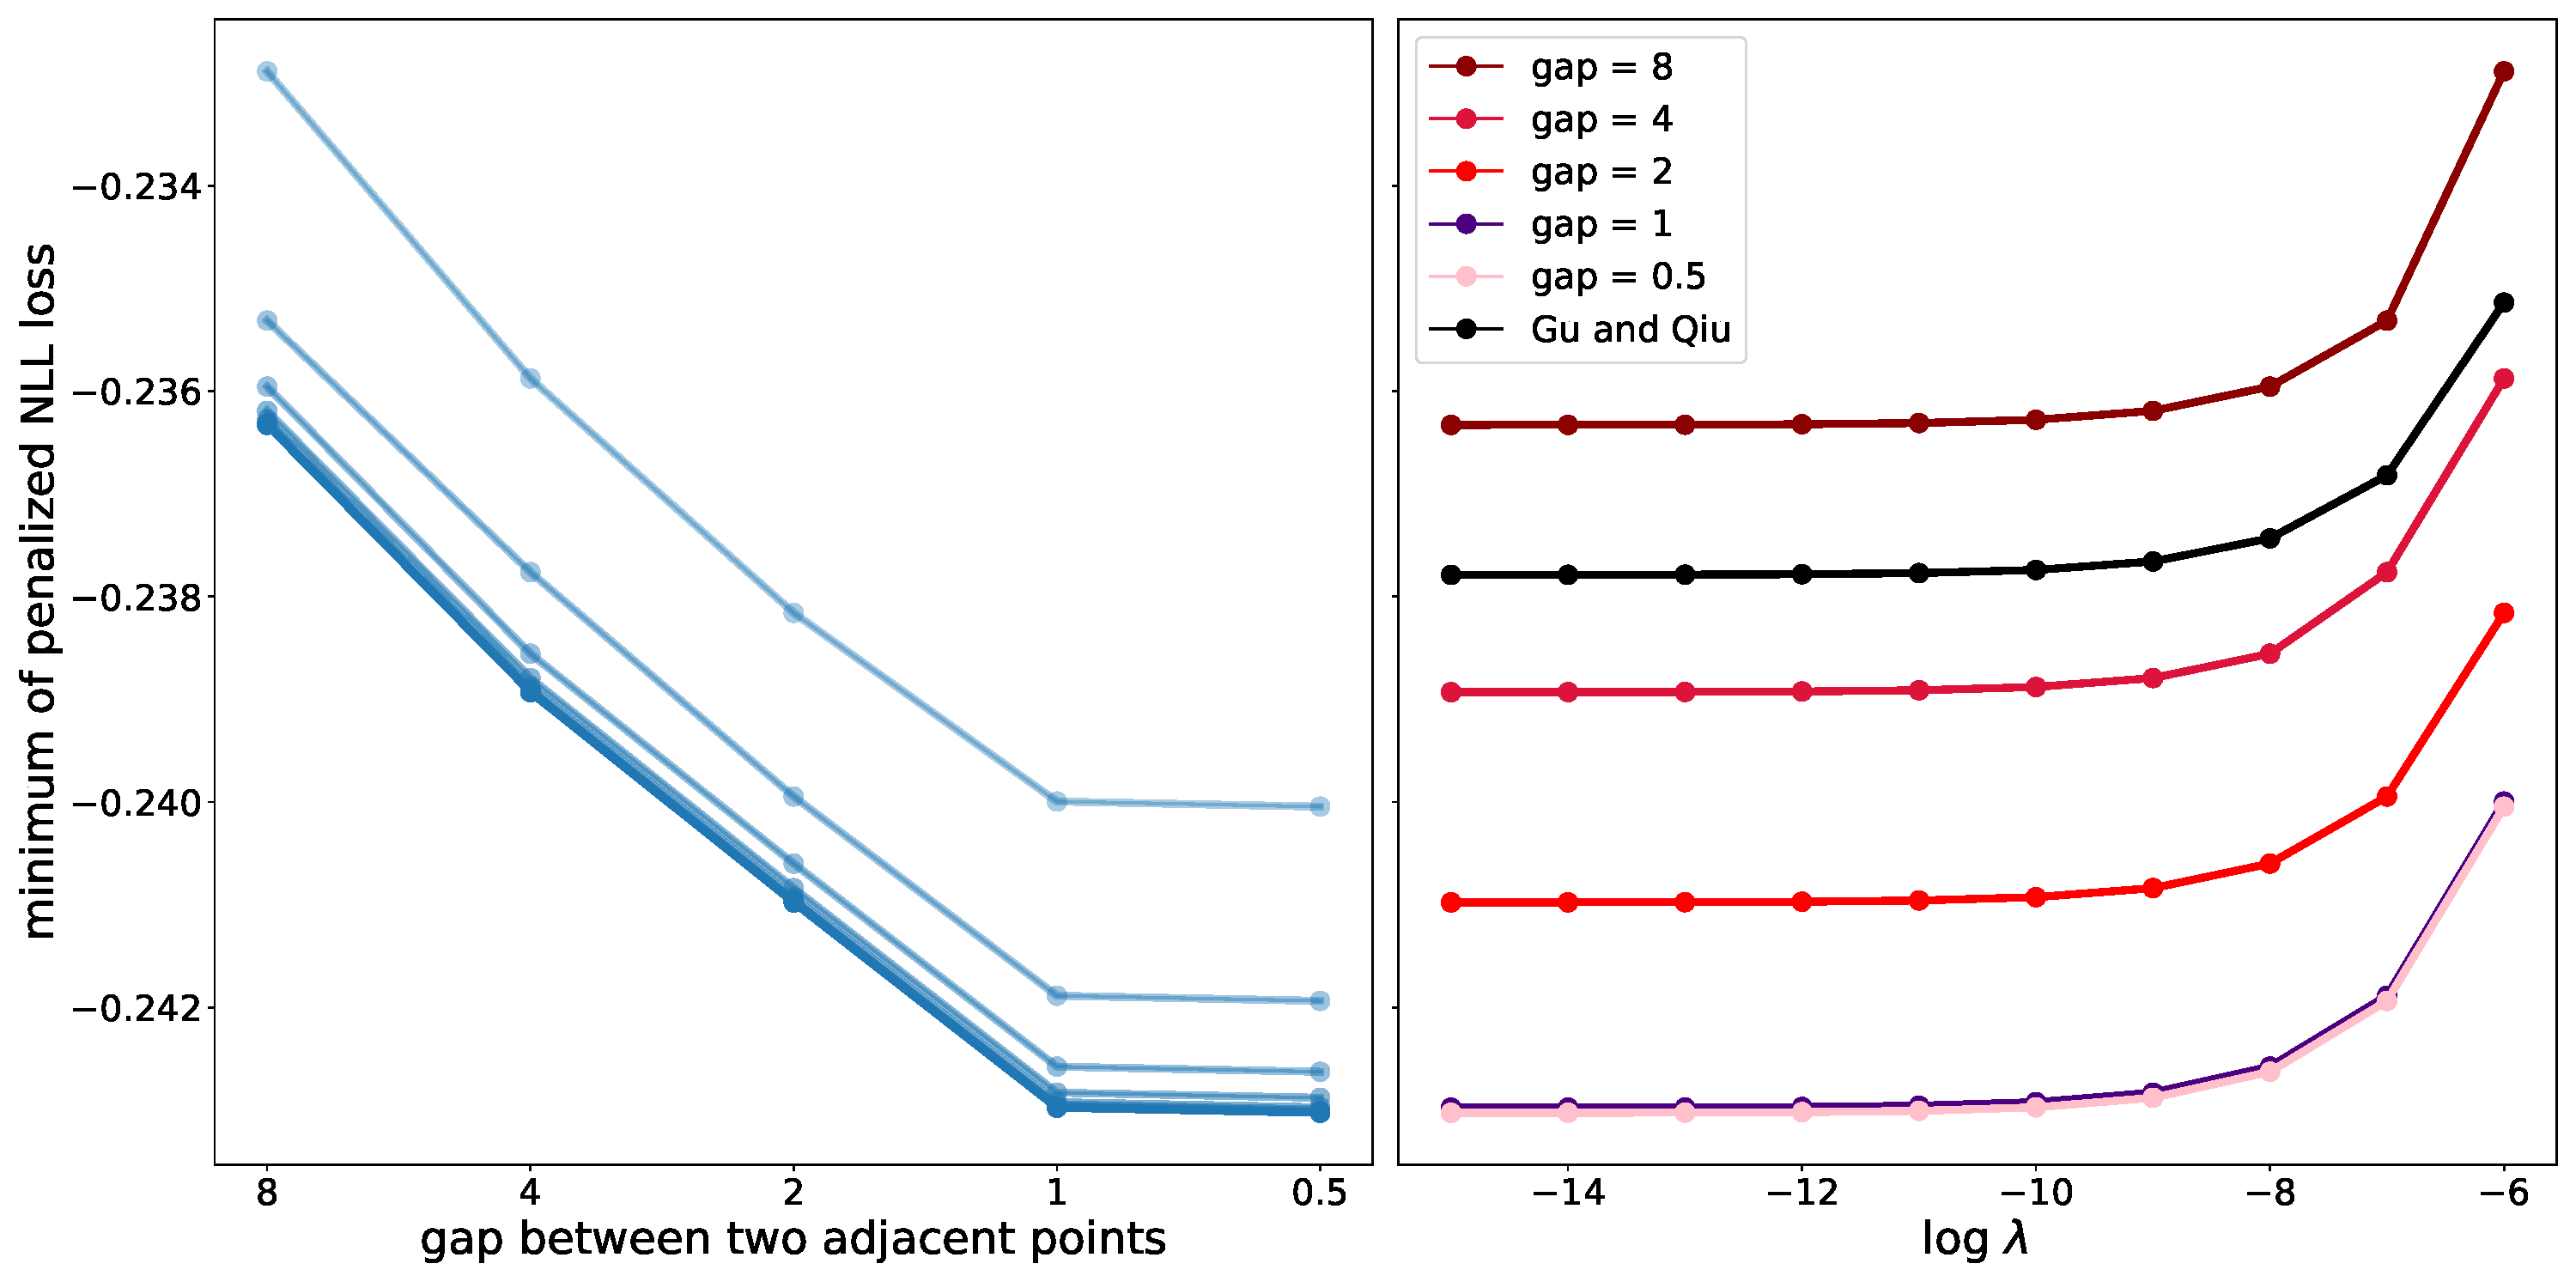
\includegraphics[width=\textwidth]{../plots/choose-best-fin-dim-approx-subspace-bw=5.0.pdf}
	\caption{Left panel: the minimum of $\widetilde{J}_{\NLL, \lambda}$ against the gap between two adjacent points at which kernel functions are centered in different choices of finite-dimensional approximating subspace. Different opacity indicates different values of $\lambda$, and the more opaque line indicates the smaller $\lambda$ value. Right panel: the minimum of $\widetilde{J}_{\NLL, \lambda}$ against different values of $\log \lambda$.}
	\label{fig-choose-fin-dim-approx-subspace}
\end{figure}

The left panel of Figure \ref{fig-choose-fin-dim-approx-subspace} shows the minimum of $\widetilde{J}_{\NLL, \lambda}$ against the gap between two adjacent grid points at which kernel functions are centered in different choices of finite-dimensional approximating subspace. For each value of $\lambda$, we see that, as the gap between two adjacent grid points becomes smaller and smaller, the minimum of $\widetilde{J}_{\NLL, \lambda}$ keeps decreasing. When the difference between two adjacent grid points is 1, if we further insert additional grid points, the further reduction on the minimum of $\widetilde{J}_{\NLL, \lambda}$ becomes negligible. Thus, for this particular \texttt{waiting} data, we use the following subspace as our final choice of the finite-dimensional approximating subspace
\begin{align}\label{eq-final-fin-dim-approx-subspace}
	\widetilde{\calH} := \sets[\Bigg]{f \biggm| f := \sum_{j=1}^{201} \beta_j k \parens{w_j, \,\cdot\,}, \beta_j \in \Real, w_j = j, \text{ for all } j = 1, \cdots, 201}. 
\end{align}

The right panel of Figure \ref{fig-choose-fin-dim-approx-subspace} shows the minimum of $\widetilde{J}_{\NLL, \lambda}$ against different values of $\log \lambda$. Similar to our observations from the left panel, as the gap between two adjacent grid points becomes smaller and smaller, the minimum of $\widetilde{J}_{\NLL, \lambda}$ keeps decreasing for all choices of $\lambda$. Comparing the minimums of $\widetilde{J}_{\NLL, \lambda}$ over the finite-dimensional subspaces with the gap between two adjacent grid points being 1 and 0.5, the difference is very tiny. In addition, the black curve in this panel shows the minimums of $\widetilde{J}_{\NLL, \lambda}$ using the finite-dimensional approximating subspace \eqref{eq-fin-approx-subspace-gu-qiu} that \textcite{Gu1993-na} and \textcite{Gu1993-lf} proposed. It is obvious that our approach yields a smaller minimum of $\widetilde{J}_{\NLL, \lambda}$ than their approach does, implying the superiority of our approach. 

\section{Regularized Score Matching Density Estimators in a Finite-dimensional Approximating Space}\label{section-computation-sm-density-estimator}

We minimize the penalized NLL loss functional over a finite-dimensional approximating space. Since our ultimate goal of this chapter is to compare the regularized SM density estimators and the penalized ML density estimator and understand their similarities and differences, in order to ensure the comparability, we also minimize the (penalized) SM loss functional over the same finite-dimensional subspace of $\calH$. We describe how to achieve this in the current section. 

Throughout this section, we again let 
\begin{align*}
	\widetilde{\calH} :=\sets[\bigg]{f \Bigm| f := \sum_{j=1}^m \beta_j k \parens{w_j, \,\cdot\,}, \beta_j \in \Real \text{ for all } j = 1, 2, \cdots, m} 
\end{align*}
be a finite-dimensional approximating subspace, where $\sets{w_1, \cdots, w_m} \subset \calX$ is a set of specified grid points. We first derive the expression of $\widehat{J}_{\SM} \parens{f}$ with $f \in \widetilde{\calH}$, where $\widehat{J}_{\SM}$ is the SM loss functional given by \eqref{eq-sm-loss-kef} in Chapter \ref{ch2}. 

\begin{proposition}\label{prop-sm-loss-fin-dim-space}
	Let $f = \sum_{j=1}^m w_j k \parens{w_j, \,\cdot\,} \in \widetilde{\calH}$. Then, the SM loss functional can be written as 
	\begin{align*}
		\widetilde{J}_{\SM} \parens{\bbeta} := \frac{1}{2} \bbeta^\top \parens[\bigg]{\frac{1}{n} \bS \bS^\top } \bbeta - \bbeta^\top \bt, 
	\end{align*}
	where $\bbeta := \parens{\beta_1, \cdots, \beta_m}^\top \in \Real^m$, the $\parens{j, \parens{i-1}d + u}$-entry of $\bS \in \Real^{m \times \parens{nd}}$ is $\innerp{k \parens{w_j, \,\cdot\,}}{\partial_u k \parens{X_i, \,\cdot\,}}_{\calH} = \partial_u k \parens{X_i, w_j}$, and the $j$-th entry of $\bt \in \Real^m$ is 
	\begin{align*}
		\innerp{\hat{z}}{k \parens{w_j, \,\cdot\,}} = - \frac{1}{n} \sum_{i=1}^n \sum_{u=1}^d \parens[\big]{\partial_u^2 k \parens{X_i, w_j} + \parens{\partial_u \log \mu} \parens{X_i} \partial_u k \parens{X_i, w_j}}, 
	\end{align*}
	for all $j = 1, \cdots, m$, $i = 1, \cdots, n$ and $u = 1, \cdots, d$. 
\end{proposition}

Proof of Proposition \ref{prop-sm-loss-fin-dim-space} can be found in Section \ref{proof-prop-sm-loss-fin-dim-space}. 

\subsection{Penalized Score Matching Density Estimator}

In order to compute the penalized SM density estimator under the constraint $f \in \widetilde{\calH}$, we minimize the penalized SM loss functional $\widehat{J}_{\SM} \parens{f} + \frac{\rho}{2} \norm{f}_{\calH}^2$ subject to $f \in \widetilde{\calH}$. The following proposition establishes the existence and the uniqueness of this minimizer, and discusses how to compute it. 

\begin{proposition}\label{prop-penalized-sm-fin-dim-space}
	The minimizer of $\widehat{J}_{\SM} \parens{f} + \frac{\rho}{2} \norm{f}_{\calH}^2$ subject to $f \in \widetilde{\calH}$, denoted by $\tilde{f}_{\SM}^{\parens{\rho}}$, exists and is unique, and is given by 
	\begin{align*}
		\tilde{f}_{\SM}^{\parens{\rho}} = \sum_{j=1}^m \beta_{j}^{\parens{\rho}} k \parens{w_j, \,\cdot\,}, 
	\end{align*}
	where $\bbeta_{\SM}^{\parens{\rho}} := \parens{\beta_{1}^{\parens{\rho}}, \beta_{2}^{\parens{\rho}}, \cdots, \beta_{m}^{\parens{\rho}}}^\top \in \Real^m$ satisfies 
	\begin{align*}
		\parens[\bigg]{\frac{1}{n} \bS \bS^\top + \lambda \bK_2} \bbeta_{\SM}^{\parens{\rho}} = \bt, 
	\end{align*}
	where $\bS \in \Real^{m \times \parens{nd}}$ and $\bt \in \Real^m$ are the same as those defined in Proposition \ref{prop-sm-loss-fin-dim-space}, and $\bK_2 \in \Real^{m \times m}$ is the same as the one used in \eqref{eq-nll-opt-problem-beta}. 
\end{proposition}

Proof of Proposition \ref{prop-penalized-sm-fin-dim-space} can be found in Section \ref{proof-prop-penalized-sm-fin-dim-space}. 

\subsection{Early Stopping Score Matching Density Estimator}

We now discuss how to compute the early stopping SM density estimator with $f \in \widetilde{\calH}$. We apply the gradient descent algorithm to minimizing $\widetilde{J}_{\SM}$ over $\Real^m$. The corresponding gradient descent iterates are 
\begin{align}\label{eq-early-stop-sm-fin-dim-space-iterate}
	\bbeta_{\SM}^{\parens{t+1}} = \bbeta_{\SM}^{\parens{t}} - \tau \bracks{ \bM \bbeta_{\SM}^{\parens{t}} - \bt } = \parens{\bI - \tau \bM} \bbeta_{\SM}^{\parens{t}} + \tau \bt, 
\end{align}
where $\bM := \frac{1}{n} \bS \bS^\top$ for notational simplicity, $\bbeta_{\SM}^{\parens{0}} \in \Real^m$ is the starting point of the algorithm, and $\tau > 0$ is the appropriately chosen constant step size. 

The following proposition links $\bbeta_{\SM}^{\parens{t}}$ to $\bbeta_{\SM}^{\parens{0}}$. 

\begin{proposition}\label{prop-early-stop-sm-fin-dim-space}
	For all $t \in \Natural_0$, we have 
	\begin{align}\label{eq-prop-early-stop-sm-fin-dim-space-1}
		\bbeta_{\SM}^{\parens{t+1}} = \parens{\bI - \tau \bM}^{t+1} \bbeta_{\SM}^{\parens{0}} + \tau \sum_{\ell=0}^{t} \parens{\bI - \tau \bM}^{\ell} \bt. 
	\end{align}
	If, in particular, we choose $\bbeta_{\SM}^{\parens{0}} = \boldzero_m$, the $m$-dimensional zero vector, we have 
	\begin{align}\label{eq-prop-early-stop-sm-fin-dim-space-2}
		\bbeta_{\SM}^{\parens{t+1}} = \tau \bQ \widetilde{\bLambda}^{\parens{t+1}} \bQ^\top \bt, \qquad \text{ for all } t \in \Natural_0, 
	\end{align}
	where $\bQ \bLambda \bQ^\top = \bM$ be the eigen-decomposition of $\bM$, $\bQ$ is an orthogonal matrix, $\bLambda$ is a diagonal matrix with all eigenvalues of $\bM$, $\lambda_1 \ge \lambda_2 \cdots \ge \lambda_m$, on the diagonal, and $\widetilde{\bLambda}^{\parens{t+1}}$ is the diagonal matrix with elements on the diagonal being 
	\begin{align*}
		\tilde{\lambda}_j^{\parens{t+1}} = \begin{cases}
			\dfrac{1 - \parens{1 - \tau \lambda_j}^{t+1}}{\tau \lambda_j}, & \, \text{ if } \lambda_j \neq 0, \\ 
			t + 1, & \, \text{ if } \lambda_j = 0, 
		\end{cases}
	\end{align*}
	for all $j = 1, \cdots, m$ and $t \in \Natural_0$. 
\end{proposition}

Proof of Proposition \ref{prop-early-stop-sm-fin-dim-space} can be found in Section \ref{proof-prop-early-stop-sm-fin-dim-space}. 

Using Proposition \ref{prop-early-stop-sm-fin-dim-space}, the $\parens{t+1}$-st gradient descent iterate of $\widehat{J}_{\SM}$ in $\widetilde{\calH}$ is 
\begin{align*}
	\sum_{j=1}^m \beta_{j}^{\parens{t+1}} k \parens{w_j, \,\cdot\,}, 
\end{align*}
where $\beta_{j}^{\parens{t+1}}$ is the $j$-th component of $\bbeta_{\SM}^{\parens{t+1}}$. 


\section{Comparison of Regularized Maximum Likelihood and Score Matching Density Estimators}\label{section-ml-sm-comparison}

With the algorithms of minimizing the penalized NLL loss functional and the (penalized) SM loss functional over a finite-dimensional approximating subspace of $\calH$ shown in the preceding sections, we now use numerical examples to compare the corresponding density estimators and understand their similarities and differences. 

\begin{sidewaysfigure}
	\centering
	
\includegraphics[width=\textwidth]{../plots/waiting-ML-vs-SM-density-estimates-baseden=Gamma-36-2-gridpoint=1-202-1-2.pdf}
	\caption{Penalized ML (first row), penalized SM (second row), and early stopping SM (third row) density estimates of the \texttt{waiting} variable. Histogram of data with the bin width chosen by the Freedman-Diaconis rule is shown in green. The rug plot indicates the location of data and the purple circle indicates the location of the isolated observation 108.}
	\label{fig-sm-ml-compare-with108}
\end{sidewaysfigure}

We again use the \texttt{waiting} variable in the Old Faithful Geyser dataset. Figure \ref{fig-sm-ml-compare-with108} shows the resulting density estimates with different choices of penalty parameters or numbers of iterations. All these density estimates are computed over the finite-dimensional subspace \eqref{eq-final-fin-dim-approx-subspace}. We use the same $\calX$, $\mu$, and $k$ as in Chapter \ref{ch3}. 

From the second and third rows of Figure \ref{fig-sm-ml-compare-with108}, we see that, similar to our findings in Chapter \ref{ch3}, two kinds of regularized SM density estimates are still qualitatively very similar. 

The penalized ML and regularized SM density estimates are qualitatively very similar when there is a large or intermediate amount of regularization. However, they are very different when there is very small regularization (small penalty parameter values or a large number of iterations). Specifically, when a very small regularization is imposed, regularized SM density estimates contains a bump or becomes a spike at the isolated observation, but penalized ML density estimates do not, even when there is no penalty (the case when $\lambda = 0$). 

\begin{sidewaysfigure}
	\centering
	
\includegraphics[width=\textwidth]{../plots/waiting-ML-vs-SM-density-estimates-baseden=Gamma-36-2-gridpoint=1-202-1-no108-2.pdf}
	\caption{Penalized ML (first row), penalized SM (second row), and early stopping SM (third row) density estimates of the \texttt{waiting} variable with the isolated observation 108 removed. Histogram of data with the bin width chosen by the Freedman-Diaconis rule is shown in green. The rug plot indicates the location of data.}
	\label{fig-sm-ml-compare-no108}
\end{sidewaysfigure}

If we remove this isolated observation 108, as is shown in Figure \ref{fig-sm-ml-compare-no108}, regularized SM density estimates do not contain a spike when the regularization is small. 

Based on these numerical examples, we conclude that the regularized SM density estimators are very sensitive to the presence of an isolated observation, especially when there is a small amount of regularization. Additional numerical examples confirm this. 


\section{Discussion on the Presence of a Spike in Score Matching Density Estimates}\label{section-sm-explanation}

We now attempt to explain why the regularized SM density estimates put a spike at the isolated observation when regularization is very small. With $d = 1$, we can write the SM loss functional as 
\begin{align*}% \label{eq-sm-loss-explain}
	\widehat{L}_{\SM} \parens{q_f} = & \, \underbrace{\frac{1}{n} \sum_{i \neq i^*} \parens[\bigg]{\frac{1}{2} \parens[\big]{ \parens{\log q_f}' \parens{X_i}}^2 + \parens{\log q_f}'' \parens{X_i}}}_{=: \parens{\mathrm{I}}} + \nonumber \\ 
	& \qquad \qquad \underbrace{\frac{1}{n} \parens[\bigg]{\frac{1}{2} \parens[\big]{ \parens{\log q_f}' \parens{X_{i^*}}}^2 + \parens{\log q_f}'' \parens{X_{i^*}}}}_{=: \parens{\mathrm{II}}}, 
\end{align*}
where $X_{i^*}$ denotes the isolated observation. 

Recall that the penalized SM density estimator is obtained by minimizing $\widehat{L}_{\SM} \parens{q_f} + \frac{\rho}{2} \norm{f}_{\calH}^2$. When $\rho$ is tiny, we are effectively minimizing the $\widehat{L}_{\SM}$ part. Notice $\log q_f$ is a linear combination of $\log \mu$ and Gaussian kernel functions centered at a set of grid points or the first two derivatives of Gaussian kernels centered at data points (depending on which basis functions we use), and these Gaussian kernel functions and derivatives of Gaussian kernel functions are local basis functions. Also, note that a spike is essentially a local maximum. Consequently, putting a spike in $\log q_f$ at $X_{i^*}$ has the effects of forcing $\parens{\parens{\log q_f}' \parens{X_{i^*}}}^2 \approx 0$ and reducing the value of $\parens{\log q_f}'' \parens{X_{i^*}}$ and, hence, that of (II) a lot, without affecting $\parens{\mathrm{I}}$ much. Thus, putting a spike at $X_{i^*}$ can reduce the value of $\widehat{L}_{\SM}$, coinciding with the goal of minimizing $\widehat{L}_{\SM}$. 

A similar explanation holds for the early stopping SM density estimator. As we keep running the gradient descent algorithm, we are searching for a $q_f \in \calQ_{\ker}$ that can reduce the value of $\widehat{L}_{\SM}$ as much as possible. With an isolated observation $X_{i^*}$ being present and local basis functions being used, putting a spike at $X_{i^*}$ can achieve this goal. 

\newpage

\section{Proofs}\label{section-proof}

\subsection{Proof of Proposition \ref{prop-nll-sol-exist-unique}}\label{proof-prop-nll-sol-exist-unique}

\begin{proof}[Proof of Proposition \ref{prop-nll-sol-exist-unique}]
	First, by \ref{assumption-2-2-bdd-kernel} in Chapter \ref{ch2}, we know $\calF = \calH$ so that minimizing \eqref{eq-pen-nll-loss} over $\calH$ is an unconstrained minimization problem. 
	
	By \ref{assumption-2-3-no-const-fun} and Theorem \ref{prop-convexity-A} in Chapter \ref{ch2}, we know $A$ is strictly convex. In addition, since $\frac{1}{n} \sum_{i=1}^n f \parens{X_i} = \frac{1}{n} \sum_{i=1}^n \innerp{f}{k \parens{X_i, \,\cdot\,}}$ is convex in $f$, we conclude $\widehat{J}_{\NLL}$ is convex. In addition, note that the functional $f \mapsto \frac{\lambda}{2} \norm{f}_{\calH}^2$ is strongly convex with constant $\lambda > 0$. It follows that the objective functional in \eqref{eq-pen-nll-loss} is strongly convex with constant $\lambda > 0$ \parencite[Proposition 10.8 in][]{Bauschke2017-he}. Finally, Corollary 11.17 in \textcite{Bauschke2017-he} implies \eqref{eq-pen-nll-loss} has exactly one minimizer in $\calH$. 
\end{proof}


\subsection{Details about Example \ref{example-representer-theorem-fails}}\label{proof-example-representer-theorem-fails}

	We provide details about Example \ref{example-representer-theorem-fails} here, and will follow three steps: 
	\begin{enumerate}
		\item[] Step 1. Identify the RKHS $\calH$ associated with the choice of $k$ and the corresponding natural parameter space $\calF$; 
		\item[] Step 2. Identify $\mathrm{Span} \sets{k \parens{X_1, \,\cdot\,}}$ and $\mathrm{Span} \sets{k \parens{X_1, \,\cdot\,}} \cap \calF$; 
		\item[] Step 3. Explcitly compute the minimizer of \eqref{eq-example-nll-representer-theorem-fails-1} over $\calF$ and show this minimizer does not reside in $\mathrm{Span} \sets{k \parens{X_1, \,\cdot\,}} \cap \calF$. 
	\end{enumerate}
	
	\underline{Step 1.} Letting $x = \parens{x_1, x_2}^\top \in \Real^2$ and $y = \parens{y_1, y_2}^\top \in \Real^2$ be arbitrary, we have 
	\begin{align*}
		k \parens{x, y} = \parens{x^\top y}^2 
		%= & \, \parens{x_1 y_1 + x_2 y_2}^2 \\ 
		= x_1^2 y_1^2 + 2 x_1 x_2 y_1 y_2 + x_2^2 y_2^2 
		= \innerp{\Phi \parens{x}}{\Phi \parens{y}}, \qquad \text{ for all } x, y \in \Real, 
%		= & \, \begin{pmatrix}
%			x_1^2 \\ \sqrt{2} x_1 x_2 \\ x_2^2
%		\end{pmatrix}^\top 
%		\begin{pmatrix}
%			y_1^2 \\ \sqrt{2} y_1 y_2 \\ y_2^2
%		\end{pmatrix} \\ 
%		= & \, \innerp[\Bigg]{\begin{pmatrix}
%			x_1^2 \\ \sqrt{2} x_1 x_2 \\ x_2^2
%		\end{pmatrix}}{\begin{pmatrix}
%			y_1^2 \\ \sqrt{2} y_1 y_2 \\ y_2^2
%		\end{pmatrix}}. 
	\end{align*}
	where $\Phi: \Real^2 \to \Real^3$ denotes the feature map of $k$ and is given by 
	\begin{align*}
		\Phi \parens{x} = \parens[\Big]{x_1^2, \sqrt{2} x_1 x_2, x_2^2}^{\top}, %\qquad \text{ for all } x = \parens{x_1, x_2} \in \Real^2, 
	\end{align*}
	and the inner product $\innerp{\,\cdot\,}{\,\cdot\,}$ is the dot product in $\Real^3$. Then, the resulting $\calH$ contains all functions mapping from $\Real^2$ to $\Real$ of the form 
	\begin{align*}
		f \parens{x} 
		%= f^\top \Phi \parens{x} = \innerp{f}{\Phi \parens{x}} 
		= w_1 x_1^2 + \sqrt{2} w_2 x_1 x_2 + w_3 x_2^2, \qquad \text{ for all } x = \parens{x_1, x_2}^\top \in \Real^2, 
	\end{align*}
	for some $w_1, w_2, w_3 \in \Real$ with the RKHS norm of $f$ being $\norm{f}_{\calH} = \sqrt{w_1^2 + w_2^2 + w_3^2}$ \parencite[Theorem 4.21 in][]{Steinwart2008-tn}. 
	
	We now derive the natural parameter space $\calF$. Let $f \parens{x} = w_1 x_1^2 + \sqrt{2} w_2 x_1 x_2 + w_3 x_2^2$ for some $w_1, w_2, w_3 \in \Real$ and all $x = \parens{x_1, x_2}^\top \in \Real^2$. By simple algebra, we have 
	\begin{align*}
		e^{A \parens{f}} = & \, \int \int_{\Real^2} \frac{1}{2\pi} \exp \parens[\bigg]{- \frac{\norm{x}_2^2}{2}} \exp \parens[\big]{f \parens{x}} \diff x_1 \diff x_2 
		%  = & \, \int \int_{\Real^2} \frac{1}{2\pi} \exp \parens[\bigg]{- \frac{x_1^2 + x_2^2}{2} + w_1 x_1^2 + \sqrt{2} w_2 x_1 x_2 + w_3 x_2^2} \diff x_1 \diff x_2 \\ 
		 % = & \, \int \int_{\Real^2} \frac{1}{2\pi} \exp \parens[\bigg]{- \frac{1}{2} \parens[\big]{x_1^2 + x_2^2 - 2 w_1 x_1^2 - 2 \sqrt{2} w_2 x_1 x_2 - 2 w_3 x_2^2}} \diff x_1 \diff x_2 \\ 
		 % = & \, \int \int_{\Real^2} \frac{1}{2\pi} \exp \parens[\bigg]{- \frac{1}{2} \parens[\big]{\parens{1 - 2 w_1} x_1^2 - 2 \sqrt{2} w_2 x_1 x_2 + \parens{1 - 2 w_3} x_2^2}} \diff x_1 \diff x_2 \\ 
		 % = & \, \int \int_{\Real^2} \frac{1}{2\pi} \exp \parens[\bigg]{- \frac{1}{2} x^\top W^{-1} x} \diff x_1 \diff x_2 \\ 
		 % = & \, \int \int_{\Real^2} \frac{\abs{W}^{1/2}}{2\pi \abs{W}^{1/2}} \exp \parens[\bigg]{- \frac{1}{2} x^\top W^{-1} x} \diff x_1 \diff x_2 \\ 
		 = \abs{W}^{1/2}, 
	\end{align*}
	where $\abs{W}$ denotes the determinant of the matrix $W$, 
	\begin{align*}
		W^{-1} = \begin{pmatrix}
			1 - 2w_1 & -\sqrt{2} w_2 \\ -\sqrt{2} w_2 & 1 - 2w_3
		\end{pmatrix}, 
	\end{align*}
	and we assume $\parens{1 - 2 w_1} \parens{1 - 2 w_3} - 2w_2^2 > 0$. Then, 
	\begin{align*}
		A \parens{f} = \log \parens[\big]{\abs{W}^{1/2}} = -\frac{1}{2} \log \parens[\big]{\parens{1 - 2w_1} \parens{1 - 2w_3} - 2 w_2^2}. 
	\end{align*}
	Note that $A \parens{f} < \infty$ if and only if $W$ is positive definite if and only if $1 - 2w_1 > 0$ and $1 - 2 w_3 > 0$ and $\parens{1 - 2w_1} \parens{1 - 2w_3} - 2 w_2^2 > 0$ if and only if $w_1 < \frac{1}{2}$ and $w_3 < \frac{1}{2}$ and $\parens{1 - 2w_1} \parens{1 - 2w_3} - 2 w_2^2 > 0$. 
	
	As the conclusion of Step 1, we have 
	\begin{align}
		\calH = & \, \bigg\{f: \Real^2 \to \Real \Bigm| f \parens{x} := w_1 x_1^2 + \sqrt{2} w_2 x_1 x_2 + w_3 x_2^2 \text{ for all } x = \parens{x_1, x_2}^\top \in \Real^2, \nonumber \\ 
		& \quad \quad \qquad \qquad \qquad w_1, w_2, w_3 \in \Real \bigg\}, \label{eq-example-nll-representer-theorem-fails-rkhs} \\ 
		\calF = & \, \bigg\{f: \Real^2 \to \Real \Bigm| f \parens{x} = w_1 x_1^2 + \sqrt{2} w_2 x_1 x_2 + w_3 x_2^2 \text{ for all } x = \parens{x_1, x_2}^\top \in \Real^2, \nonumber \\ 
		& \quad \qquad \qquad \qquad \quad w_1 < \frac{1}{2}, w_3 < \frac{1}{2}, \parens{1 - 2w_1} \parens{1 - 2w_3} - 2 w_2^2 > 0, w_1, w_2, w_3 \in \Real \bigg\}. \label{eq-example-nll-representer-theorem-fails-F}
	\end{align}
	
	\underline{Step 2.} With $X_1 = \parens{a, 0}^\top$, it is easy to see $\mathrm{Span} \sets{k \parens{X_1, \,\cdot\,}}$ contains all functions of the form 
	\begin{align*}
		f \parens{x} = \gamma k \parens{X_1, x} = \gamma \parens{X_1^\top x}^2 = \gamma a^2 x_1^2, \quad \text{ for all } x := \parens{x_1, x_2}^\top \in \Real^2 \text{ and } \gamma \in \Real. 
	\end{align*}
	Then, we can characterize $\mathrm{Span} \sets{k \parens{X_1, \,\cdot\,}} \cap \calF$ as 
	\begin{align*}
		\mathrm{Span} \sets{k \parens{X_1, \,\cdot\,}} \cap \calF = \bigg\{f: \Real^2 \to \Real \Bigm| f \parens{x} = \gamma a^2 x_1^2 \text{ for all } x = \parens{x_1, x_2}^\top \in \Real^2, \gamma a^2 < \frac{1}{2} \bigg\}. 
	\end{align*}
	
	\underline{Step 3.} Let $f \in \calF$ be 
	\begin{align*}
		f \parens{x} = w_1 x_1^2 + \sqrt{2} w_2 x_1 x_2 + w_3 x_2^2, \qquad \text{ for all } x = \parens{x_1, x_2}^\top \in \Real^2, 
	\end{align*}
	where $w_1, w_2, w_3 \in \Real$ satisfy the constraints in \eqref{eq-example-nll-representer-theorem-fails-F}. Then, with $\lambda > 0$, $\widehat{J}_{\NLL} \parens{f} + \frac{\lambda}{2} \norm{f}_{\calH}^2$ becomes  
	\begin{align*}
		\widetilde{J}_{\lambda} \parens{w_1, w_2, w_3} := & \, - \frac{1}{2} \log \parens[\big]{\parens{1 - 2w_1} \parens{1 - 2w_3} - 2 w_2^2} - w_1 a^2 + \frac{\lambda}{2} \parens{w_1^2 + w_2^2 + w_3^2}. 
	\end{align*}
	By calculus, we have 
	\begin{align*}
		\nabla \widetilde{J}_{\lambda} \parens{w_1, w_2, w_3} = & \, \begin{pmatrix}
			\frac{1 - 2w_3}{\parens{1-2w_1} \parens{1-2w_3} - 2w_2^2} - a^2 + \lambda w_1 \\ 
			\frac{2w_2}{\parens{1-2w_1} \parens{1-2w_3} - 2w_2^2} + \lambda w_2 \\
			\frac{1 - 2w_1}{\parens{1-2w_1} \parens{1-2w_3} - 2w_2^2} + \lambda w_3
		\end{pmatrix}.  
	\end{align*}
	Any stationary points, denoted by $\parens{w_1^*, w_2^*, w_3^*}$, must satisfy $\nabla \widetilde{J}_{\lambda} \parens{w_1^*, w_2^*, w_3^*} = 0$, from which we obtain the following system of equations 
	\begin{align*}
		\begin{cases}
			\parens{1 - 2 w_3^*} + \parens{\lambda w_1^* - a^2} \parens[\big]{\parens{1 - 2w_1^*} \parens{1 - 2w_3^*} - 2{w_2^*}^2} & = 0, \\ 
			2 w_2^* + \lambda w_2^* \parens[\big]{\parens{1 - 2 w_1^*} \parens{1 - 2 w_3^*} - 2 {w_2^*}^2} & = 0, \\ 
			\parens{1 - 2 w_1^*} + \lambda w_3^* \parens[\big]{\parens{1 - 2w_1^*} \parens{1 - 2w_3^*} - 2{w_2^*}^2} & = 0. 
		\end{cases}	
	\end{align*}
	Solving the preceding system for $\parens{w_1^*, w_2^*, w_3^*}$ yields the following solutions: 
	\begin{align}\label{eq-example-all-sol}
		\parens[\bigg]{\frac{1}{2}, \, 0, \, \frac{1}{2}}, \quad \parens[\big]{b_1^*, \, 0, \, c_1^*}, \quad \parens[\big]{b_1^*, \, 0, \, c_2^*}, \quad \parens[\big]{b_2^*, \, 0, \, c_1^*}, \quad \parens[\big]{b_2^*, \, 0, \, c_2^*}, 
	\end{align}
	where 
	\begin{align*}
		& \, b_1^* := \frac{\parens{\lambda + 2 a^2} + \sqrt{\parens{\lambda - 2 a^2}^2 + 8 \lambda}}{4 \lambda}, 
		&& \, b_2^* := \frac{- \parens{\lambda + 2 a^2} + \sqrt{\parens{\lambda - 2 a^2}^2 + 8 \lambda}}{-4 \lambda}, \\ 
		& \, c_1^* := \frac{\lambda + \sqrt{\lambda^2 + 8 \lambda}}{4 \lambda}, 
		&& \, c_2^* := \frac{\lambda - \sqrt{\lambda^2 + 8 \lambda}}{4 \lambda}. 
	\end{align*}
	We next check whether the corresponding functions belong to $\calF$ or not. 
	
	First, notice that the pair of $\parens{w_1^*, w_2^*, w_3^*} = \parens{\frac{1}{2}, 0, \frac{1}{2}}$ leads to the function $f \parens{x} = \frac{1}{2} \parens{x_1^2 + x_2^2}$, which does \textit{not} belong to $\calF$ since $w_1^* = \frac{1}{2}$ and $w_3^* = \frac{1}{2}$. We discard it. 
	
	In addition, since $\lambda > 0$, we have 
	\begin{align*}
		b_1^* = \frac{\parens{\lambda + 2 a^2} + \sqrt{\parens{\lambda - 2 a^2}^2 + 8 \lambda}}{4 \lambda} > \frac{\parens{\lambda + 2 a^2} + \abs{\lambda - 2 a^2}}{4 \lambda}. 
	\end{align*}
	Consider the following two cases: 
	\begin{enumerate}
		\item[(i)] If $2 a^2 - \lambda \ge 0$, that is, $a^2/\lambda \ge \frac{1}{2}$, we have $b_1^* > \frac{\lambda + 2 a^2 + 2 a^2 - \lambda}{4 \lambda} = \frac{a^2}{\lambda} \ge \frac{1}{2}$; 

		\item[(ii)] If $2 a^2 - \lambda < 0$, we have $b_1^* > \frac{\lambda + 2 a^2 + \lambda - 2 a^2}{4 \lambda} = \frac{2\lambda}{4\lambda} \ge \frac{1}{2}$. 
	\end{enumerate}
	In both cases, we have $b_1^* > \frac{1}{2}$, and any function $f$ with $w_1^* = b_1^*$ cannot belong to $\calF$. 
	
	Next, we show $b_2^* < \frac{1}{2}$, which is equivalent to showing $1 - 2b_2^* > 0$. Since 
	\begin{align*}
		1 - 2b_2^* = & \, 1 - \frac{- \parens{\lambda + 2 a^2} + \sqrt{\parens{\lambda - 2 a^2}^2 + 8 \lambda}}{-2 \lambda} \\ 
		= & \, 1 + \frac{\sqrt{\parens{\lambda - 2 a^2}^2 + 8 \lambda} - \parens{\lambda + 2 a^2}}{2 \lambda} \\ 
		> & \, 1 + \frac{\abs{\lambda - 2 a^2} - \parens{\lambda + 2 a^2}}{2 \lambda}. 
	\end{align*}
	Again, we consider the following two cases: 
	\begin{enumerate}
		\item[(i)] If $2 a^2 - \lambda \ge 0$, we have $1 - 2 b_2^* > 1 + \frac{2 a^2 - \lambda - \lambda - 2a^2}{2 \lambda} = 1 + \frac{- 2\lambda }{2 \lambda} = 0$; 
		\item[(ii)] If $2 a^2 - \lambda < 0$, that is, $0 \le a^2 / \lambda < \frac{1}{2}$, we have $1 - 2b_2^* > 1 + \frac{\lambda - 2 a^2 - \lambda - 2 a^2}{2 \lambda} = 1 - \frac{2 a^2}{\lambda} > 0$. 
	\end{enumerate}
	
	As for $c_1^*$ and $c_2^*$, since $\lambda > 0$, we have 
	\begin{align*}
		c_1^* = & \, \frac{\lambda + \sqrt{\lambda^2 + 8 \lambda}}{4 \lambda} > \frac{\lambda + \sqrt{\lambda^2}}{4 \lambda} = \frac{1}{2}, \\ 
		c_2^* = & \, \frac{\lambda - \sqrt{\lambda^2 + 8 \lambda}}{4 \lambda} < \frac{\lambda}{4 \lambda} = \frac{1}{4} < \frac{1}{2}. 
	\end{align*}
	That is, any function $f$ with $w_3^* = c_1^*$ cannot belong to $\calF$. 
	
	As a conclusion, the only solution in \eqref{eq-example-all-sol} such that the resulting $f$ belongs to $\calF$ is $\parens{w_1^*, w_2^*, w_3^*} = \parens{b_2^*, 0, c_2^*}$. 
	
	In addition, it is easy to see that the Hessian matrix of $\widetilde{J}_{\lambda}$ at $\parens{w_1^*, w_2^*, w_3^*} = \parens{b_2^*, 0, c_2^*}$ is 
	\begin{align*}
		\begin{pmatrix}
			\frac{2 \parens{1 - c_2^*}^2}{\parens{1 - 2b_2^*}^2 \parens{1 - 2c_2^*}^2} + \lambda & 0 & 0 \\ 
			0 & \frac{2 \parens{1 - b_2^*} \parens{1 - c_2^*}}{\parens{1 - 2b_2^*}^2 \parens{1 - 2c_2^*}^2} + \lambda & 0 \\ 
			0 & 0 & \frac{2 \parens{1 - b_2^*}^2}{\parens{1 - 2b_2^*}^2 \parens{1 - 2c_2^*}^2} + \lambda
		\end{pmatrix}, 
	\end{align*}
	which is positive definite. We conclude that $\widetilde{J}_{\lambda}$ achieves the minimum at $\parens{w_1^*, w_2^*, w_3^*} = \parens{b_2^*, 0, c_2^*}$, and the corresponding function, $f^* := \argmin_{f \in \calF} \braces[\big]{\widehat{J}_{\NLL} \parens{f} + \frac{\lambda}{2} \norm{f}_{\calH}^2}$, is 
	\begin{align*}% \label{ex.optf}
		f^* \parens{x} = b_2^* x_1^2 + c_2^* x_2^2, \qquad \text{ for all } x = \parens{x_1, x_2}^\top \in \Real^2. 
	\end{align*}
	Since $c_2^* \neq 0$ for all $\lambda > 0$, $f^*$ does \emph{not} belong to $\mathrm{Span} \sets{k \parens{X_1, \,\cdot\,}} \cap \calF$. \hfill \qedsymbol


\subsection{Proof of Proposition \ref{prop-sm-loss-fin-dim-space}}\label{proof-prop-sm-loss-fin-dim-space}

\begin{proof}[Proof of Proposition \ref{prop-sm-loss-fin-dim-space}]
	Since $f \in \widetilde{\calH}$ takes on the form $f = \sum_{j=1}^m \beta_j k \parens{w_j, \,\cdot\,}$ for $\beta_1, \cdots, \beta_m \in \Real$, we first have 
	\begin{align*}
		& \, \innerp{f}{\parens{\partial_u k \parens{X_i, \,\cdot\,} \otimes \partial_u k \parens{X_i, \,\cdot\,}} f}_{\calH} \nonumber \\ 
		= & \, \innerp[\bigg]{\sum_{\ell=1}^m \beta_{\ell} k \parens{w_\ell, \,\cdot\,}}{\parens{\partial_u k \parens{X_i, \,\cdot\,} \otimes \partial_u k \parens{X_i, \,\cdot\,}} \parens[\bigg]{\sum_{j=1}^m \beta_j k \parens{w_j, \cdot}}}_{\calH} \nonumber \\ 
		% = & \, \sum_{\ell=1}^m \sum_{j=1}^m \alpha_{\ell} \alpha_j \innerp[\big]{k \parens{w_\ell, \cdot}}{\parens{\partial_u k \parens{X_i, \cdot} \otimes \partial_u k \parens{X_i, \cdot}} k \parens{w_j, \cdot}}_{\calH} \nonumber \\ 
		= & \, \sum_{\ell=1}^m \sum_{j=1}^m \beta_{\ell} \beta_j \innerp{\partial_u k \parens{X_i, \,\cdot\,}}{k \parens{w_\ell, \,\cdot\,}}_{\calH} \innerp{\partial_u k \parens{X_i, \,\cdot\,}}{k \parens{w_j, \,\cdot\,}}_{\calH} \nonumber \\ 
		= & \, \sum_{\ell=1}^m \sum_{j=1}^m \beta_{\ell} \beta_j \partial_u k \parens{X_i, w_\ell} \partial_u k \parens{X_i, w_j}, 
	\end{align*}
	where the last equality is due to the reproducing property of the partial derivative of $k$ (see Proposition \ref{prop-reproducing-derivative} in Appendix \ref{app1}). Then, since $\widehat{C} = \frac{1}{n} \sum_{i=1}^n \sum_{u=1}^d \partial_u k \parens{X_i, \,\cdot\,} \otimes \partial_u k \parens{X_i, \,\cdot\,}$, by the linearity of the inner product, we have 
	\begin{align*}
		\innerp{f}{\widehat{C} f}_{\calH} = & \, \frac{1}{n} \sum_{i=1}^n \sum_{u=1}^d \innerp[\big]{f}{\parens{\partial_u k \parens{X_i, \cdot} \otimes \partial_u k \parens{X_i, \cdot}} f}_{\calH} \nonumber \\ 
		= & \, \frac{1}{n} \sum_{i=1}^n \sum_{u=1}^d \sum_{\ell=1}^m \sum_{j=1}^m \beta_{\ell} \beta_j \partial_u k \parens{X_i, w_\ell} \partial_u k \parens{X_i, w_j} \\ 
		% = & \, \bbeta^\top \parens[\bigg]{\frac{1}{n} \sum_{i=1}^n \sum_{u=1}^d \bg_{\parens{i - 1}d + u} \bg_{\parens{i - 1}d + u}^\top } \bbeta \nonumber \\ 
		= & \, \bbeta^\top \parens[\bigg]{\frac{1}{n} \bS \bS^\top } \bbeta. 
	\end{align*}
%	where 
%	\begin{align}
%		\bg_{\parens{i-1}d+u} = \begin{pmatrix}
%			\partial_u k \parens{X_i, w_1}, 
%			\partial_u k \parens{X_i, w_2}, 
%			\cdots, 
%			\partial_u k \parens{X_i, w_m}
%		\end{pmatrix}^\top \in \Real^m, 
%	\end{align}
%	for all $i = 1, \cdots, n$ and $u = 1, \cdots, d$, and 
%	\begin{align}
%		\bG = \begin{pmatrix}
%			\bg_1 \, \vdots \, \bg_2 \, \vdots \, \cdots \, \vdots \, \bg_{nd}
%		\end{pmatrix} \in \Real^{m \times \parens{nd}}. 
%	\end{align}

	As for $\innerp{f}{\hat{z}}_{\calH}$, we have the following 
	\begin{align*}
		\innerp{f}{\hat{z}}_{\calH} = & \, \innerp[\bigg]{\sum_{j=1}^m \beta_j k \parens{w_j, \,\cdot\,}}{- \frac{1}{n} \sum_{i=1}^n \sum_{u=1}^d \parens[\big]{\partial_u^2 k \parens{X_i, \,\cdot\,} + \parens{\partial_u \log \mu} \parens{X_i} \partial_u k \parens{X_i, \,\cdot\,}}}_{\calH} \\ 
		= & \, \sum_{j=1}^m \beta_j \parens[\bigg]{- \frac{1}{n} \sum_{i=1}^n \sum_{u=1}^d \parens[\big]{\partial_u^2 k \parens{X_i, w_j} + \parens{\partial_u \log \mu} \parens{X_i} \partial_u k \parens{X_i, w_j}} } \\ 
		= & \, \bbeta^\top \bt, 
	\end{align*}
	where we use the reproducing property of the partial derivative of $k$ in the second equality. The desired result follows by combining all pieces above together. 
\end{proof}


\subsection{Proof of Proposition \ref{prop-penalized-sm-fin-dim-space}}\label{proof-prop-penalized-sm-fin-dim-space}

\begin{proof}[Proof of Proposition \ref{prop-penalized-sm-fin-dim-space}]
	Recall from Chapters \ref{ch2} and \ref{ch3} that the operator $\widehat{C}: \calH \to \calH$ is positive semidefinite, $\widehat{J}_{\SM}$ is convex over $\calH$. In addition, note that the functional $f \mapsto \frac{\rho}{2} \norm{f}_{\calH}^2$ is strongly convex with constant $\rho$. We conclude that the penalized SM loss functional $f \mapsto \widehat{J}_{\SM} \parens{f} + \frac{\rho}{2} \norm{f}_{\calH}^2$ is strongly convex with parameter $\lambda > 0$, and that it has exactly one minimizer \parencite[Corollary 11.17 in][]{Bauschke2017-he}. 
	
	With $f = \sum_{j=1}^m \beta_j k \parens{w_j, \,\cdot\,} \in \widetilde{\calH}$, we have $\frac{\rho}{2} \norm{f}_{\calH}^2 = \frac{\rho}{2} \bbeta^\top \bK_2 \bbeta$. Thus, together with Proposition \ref{prop-sm-loss-fin-dim-space}, we can write the functional $\widehat{J}_{\SM} \parens{f} + \frac{\rho}{2} \norm{f}_{\calH}^2$ with $f \in \widetilde{\calH}$ as 
	\begin{align*}
		\widetilde{J}_{\SM, \rho} \parens{\bbeta} := \frac{1}{2} \bbeta^\top \parens[\bigg]{\frac{1}{n} \bS \bS^\top} \bbeta - \bbeta^\top \bt + \frac{\rho}{2} \bbeta^\top \bK_2 \bbeta. 
	\end{align*}
	Then, $\bbeta_{\SM}^{\parens{\rho}} := \argmin_{\bbeta \in \Real^m} \widetilde{J}_{\SM, \rho} \parens{\bbeta}$ must satisfy the first-order optimality condition 
	\begin{align*}
		\parens[\bigg]{\frac{1}{n} \bS \bS^\top + \rho \bK_2} \bbeta_{\SM}^{\parens{\rho}} = \bt. 
	\end{align*}
	As a consequence, $\argmin_{f \in \widetilde{\calH}} \sets[\big]{\widehat{J}_{\SM} \parens{f} + \frac{\rho}{2} \norm{f}_{\calH}^2}$ is $\sum_{j=1}^m \beta_j^{\parens{\rho}} k \parens{w_j, \,\cdot\,}$, where $\beta_j^{\parens{\rho}}$ is the $j$-th element of $\bbeta_{\SM}^{\parens{\rho}}$. 
\end{proof}


\subsection{Proof of Proposition \ref{prop-early-stop-sm-fin-dim-space}}\label{proof-prop-early-stop-sm-fin-dim-space}

\begin{proof}[Proof of Proposition \ref{prop-early-stop-sm-fin-dim-space}]
	We first prove \eqref{eq-prop-early-stop-sm-fin-dim-space-1} by induction. When $t = 0$, from \eqref{eq-early-stop-sm-fin-dim-space-iterate}, we have 
	\begin{align}\label{eq-prop-early-stop-sm-fin-dim-space-3}
		\bbeta_{\SM}^{\parens{1}} = \parens{\bI - \tau \bM} \bbeta_{\SM}^{\parens{0}} + \tau \bt. 
	\end{align}
	From \eqref{eq-prop-early-stop-sm-fin-dim-space-1}, we plug in $t=0$ and obtain 
	\begin{align*}
		\bbeta_{\SM}^{\parens{1}} = & \, \parens{\bI - \tau \bM} \bbeta_{\SM}^{\parens{0}} + \tau \sum_{\ell=0}^{0} \parens{\bI - \tau \bM}^i \bt 
		= \parens{\bI - \tau \bM} \bbeta_{\SM}^{\parens{0}} + \tau \bt, 
	\end{align*}
	which is identical to \eqref{eq-prop-early-stop-sm-fin-dim-space-3}. 
	
	Now, supposing \eqref{eq-prop-early-stop-sm-fin-dim-space-1} holds for $t = s$, we are going to show it also holds for $t = s+1$. Note the following 
	\begin{align}
		\bbeta_{\SM}^{\parens{s+1}} = & \, \parens{\bI - \tau \bM} \bbeta_{\SM}^{\parens{s}} + \tau \bt \nonumber \\ 
		= & \, \parens{\bI - \tau \bM} \bracks[\bigg]{\parens{\bI - \tau \bM}^s \bbeta_{\SM}^{\parens{0}} + \tau \sum_{\ell=0}^{s-1} \parens{\bI - \tau \bM}^{\ell} \bt } + \tau \bt \nonumber \\ 
		= & \, \parens{\bI - \tau \bM}^{s+1} \bbeta_{\SM}^{\parens{0}} + \tau \sum_{\ell=0}^{s-1} \parens{\bI - \tau \bM}^{\ell+1} \bt + \tau \bt \nonumber \\ 
		= & \, \parens{\bI - \tau \bM}^{s+1} \bbeta_{\SM}^{\parens{0}} + \tau \sum_{\ell=1}^{s} \parens{\bI - \tau \bM}^{\ell} \bt + \tau \bt \nonumber \\ 
		= & \, \parens{\bI - \tau \bM}^{s+1} \bbeta_{\SM}^{\parens{0}} + \tau \sum_{\ell=0}^{s} \parens{\bI - \tau \bM}^{\ell} \bt, \nonumber
	\end{align}
	which is the desired result. 
	
	We now prove \eqref{eq-prop-early-stop-sm-fin-dim-space-2}. With $\bbeta_{\SM}^{\parens{0}} = \boldzero_m$, we can simplify \eqref{eq-prop-early-stop-sm-fin-dim-space-1} to 
\begin{align*}% \label{eq-prop}
	\bbeta_{\SM}^{\parens{t+1}} = \tau \sum_{\ell=0}^{t} \parens{\bI - \tau \bM}^{\ell} \bt, \qquad \text{ for all } t \in \Natural_0. 
\end{align*}
	Let $\bQ \bLambda \bQ^\top = \bM$ be the eigen-decomposition of $\bM$, where $\bQ$ and $\bLambda$ are defined in the proposition. Then, 
\begin{align*}
	\bI - \tau \bM = \bI - \tau \bQ \bLambda \bQ^\top = \bQ \bQ^\top - \tau \bQ \bLambda \bQ^\top = \bQ \parens{\bI - \tau \bLambda} \bQ^\top, 
\end{align*}
and we have 
\begin{align*}
	\sum_{\ell=0}^{t} \parens{\bI - \tau \bM}^{\ell} = \sum_{\ell=0}^{t} \bQ \parens{\bI - \tau \bLambda}^{\ell} \bQ^\top = \bQ \bracks[\Bigg]{\sum_{\ell=0}^{t} \parens{\bI - \tau \bLambda}^{\ell}} \bQ^\top. 
\end{align*}
Now, if $\lambda_j \neq 0$, we have 
\begin{align}\label{eq-lam1}
	\sum_{\ell=0}^{t} \parens{1 - \tau \lambda_j}^{\ell} = \frac{1 - \parens{1 - \tau \lambda_j}^{t+1}}{\tau \lambda_j}; 
\end{align}
and if $\lambda_j = 0$, we have 
\begin{align}\label{eq-lam2}
	\sum_{\ell=0}^{t} \parens{1 - \tau \lambda_j}^{\ell} = t + 1. 
\end{align}

Therefore, if we let $\widetilde{\bLambda}^{\parens{t+1}}$ be the diagonal matrix with elements on the diagonal being \eqref{eq-lam1} and \eqref{eq-lam2}, the desired result follows. 
\end{proof}
